\documentclass[border=2pt]{standalone}
\usepackage{tikz}
\usepackage{amsmath}
\usepackage{mathtools}
\usepackage{adjustbox}
\usetikzlibrary{patterns}
\usetikzlibrary{calc} \usetikzlibrary{positioning} \usetikzlibrary{shapes,arrows} \usetikzlibrary{plotmarks}
\usetikzlibrary{positioning,decorations.pathreplacing}

\begin{document}

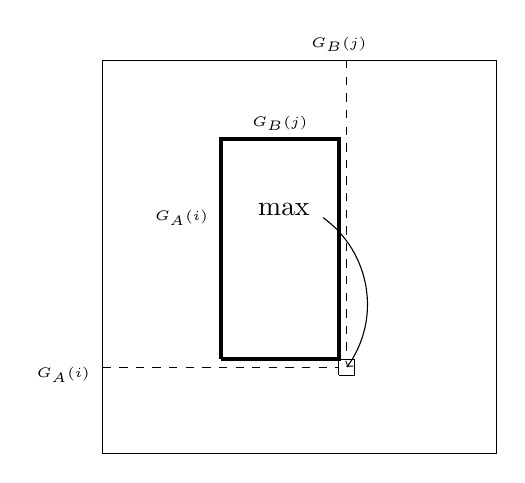
\begin{tikzpicture}
\draw (0,0) -- (5,0) -- (5,5) -- (0,5) -- (0,0);
\draw (3,1) -- (3.2,1) -- (3.2,1.2) -- (3,1.2) -- (3,1);

\node[] at (-0.5, 1) {\tiny $G_A(i)$};
\node[] at (3, 5.2) {\tiny $G_B(j)$};

\draw[line width=0.5mm] (1.5, 1.2) -- (3,1.2) -- (3, 4) -- (1.5, 4) -- (1.5, 1.2);

\node[] at (1, 3) {\tiny $G_A(i)$};
\node[] at (2.25, 4.2) {\tiny $G_B(j)$};

\draw[dashed] (0, 1.1) -- (3, 1.1);
\draw[dashed] (3.1, 5) -- (3.1, 1.2);

\node[] at (2.3, 3.1) {$\max$};

\path[solid,->](2.8, 3) edge [bend left=45]  (3.1, 1.1);

\end{tikzpicture}

\end{document}